\documentclass[tikz,border=15pt]{standalone}
\usepackage{tikz}
\usepackage{amsmath}
\usepackage{amssymb}
\usetikzlibrary{shapes.geometric, arrows.meta, positioning, calc, backgrounds, fit, shadows.blur}

\definecolor{navyDark}{HTML}{0B2545}
\definecolor{navyLight}{HTML}{F0F4F8}
\definecolor{navyBorder}{HTML}{134074}

\definecolor{crimsonDark}{HTML}{78281F}
\definecolor{crimsonLight}{HTML}{FDF2E9}
\definecolor{crimsonBorder}{HTML}{C0392B}

\definecolor{emeraldDark}{HTML}{0E6251}
\definecolor{emeraldLight}{HTML}{E8F8F5}
\definecolor{emeraldBorder}{HTML}{16A085}

\definecolor{purpleDark}{HTML}{512E5F}
\definecolor{purpleLight}{HTML}{F4ECF7}
\definecolor{purpleBorder}{HTML}{8E44AD}

\definecolor{amberDark}{HTML}{7D6608}
\definecolor{amberLight}{HTML}{FEF9E7}
\definecolor{amberBorder}{HTML}{D4AC0D}

\definecolor{slateDark}{HTML}{2C3E50}
\definecolor{slateLight}{HTML}{F8F9FA}
\definecolor{slateBorder}{HTML}{BDC3C7}

\begin{document}
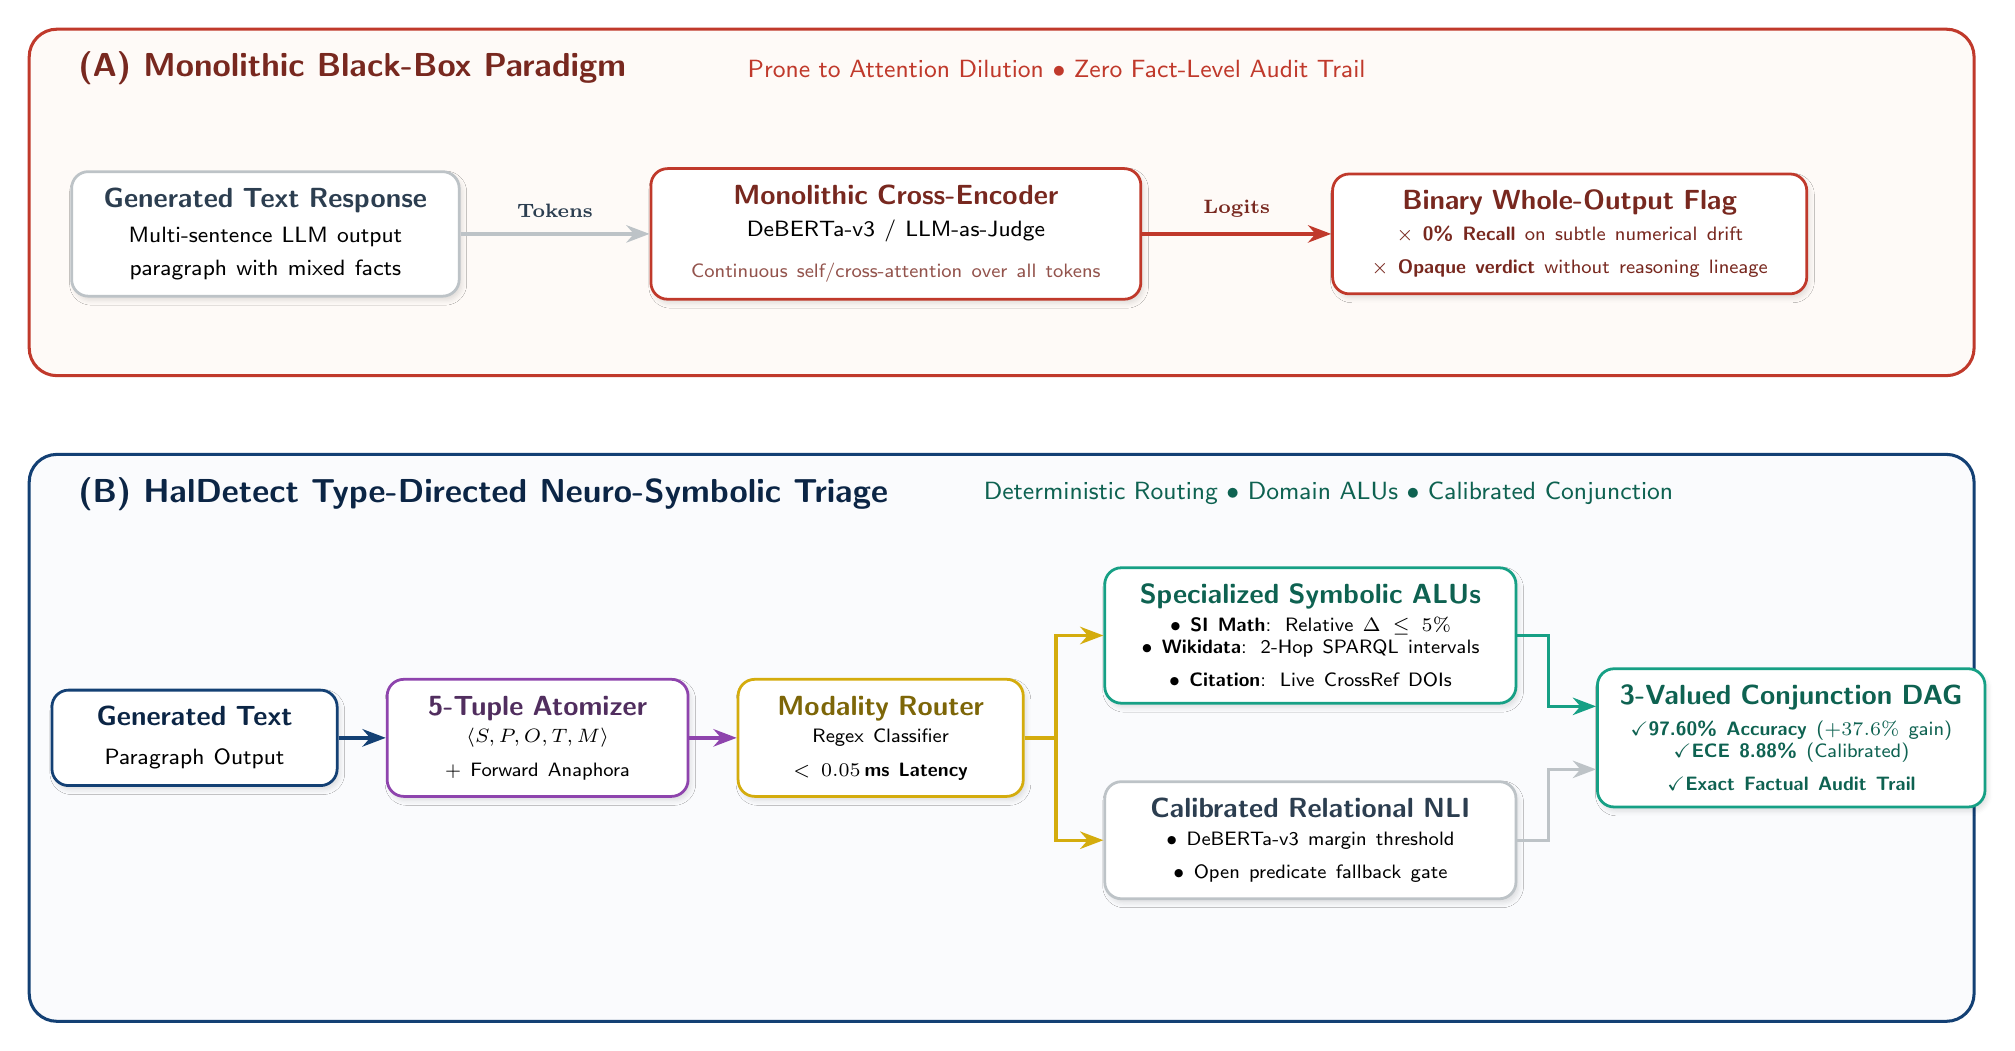
\begin{tikzpicture}[
    font=\sffamily,
    >=Stealth,
    trackbox/.style={
        draw=#1Border, fill=#1Light!35, line width=1.1pt, rounded corners=10pt
    },
    card/.style={
        draw=#1Border, fill=white, line width=1.0pt, rounded corners=6pt,
        blur shadow={shadow blur steps=4, shadow xshift=1pt, shadow yshift=-1.5pt, shadow opacity=12},
        align=center, inner sep=6pt
    },
    wire/.style={
        ->, line width=1.2pt, draw=#1Border
    }
]

% ==================== PARADIGM A: MONOLITHIC BLACK-BOX ====================
\draw[trackbox=crimson] (-0.5, 3.4) rectangle (24.2, 7.8);
\node[anchor=west, font=\sffamily\bfseries\large, text=crimsonDark] at (0.0, 7.3) {(A) Monolithic Black-Box Paradigm};
\node[anchor=west, font=\sffamily\small, text=crimsonBorder] at (8.5, 7.3) {Prone to Attention Dilution $\bullet$ Zero Fact-Level Audit Trail};

\node[card=slate, minimum width=4.8cm, text width=4.5cm] (a_in) at (2.5, 5.2) {
    \textbf{\color{slateDark} Generated Text Response}\\
    \vspace{3pt}
    \footnotesize Multi-sentence LLM output\\
    \footnotesize paragraph with mixed facts
};

\node[card=crimson, right=2.4cm of a_in, minimum width=6.2cm, text width=5.8cm] (a_enc) {
    \textbf{\color{crimsonDark} Monolithic Cross-Encoder}\\
    \vspace{2pt}
    \footnotesize DeBERTa-v3 / LLM-as-Judge\\
    \vspace{3pt}
    \scriptsize \textcolor{crimsonDark!80}{Continuous self/cross-attention over all tokens}
};

\node[card=crimson, right=2.4cm of a_enc, minimum width=6.0cm, text width=5.6cm] (a_out) {
    \textbf{\color{crimsonDark} Binary Whole-Output Flag}\\
    \vspace{3pt}
    \scriptsize \textcolor{crimsonDark}{$\times$ \textbf{0\% Recall} on subtle numerical drift}\\
    \scriptsize \textcolor{crimsonDark}{$\times$ \textbf{Opaque verdict} without reasoning lineage}
};

\draw[wire=slate] (a_in) -- (a_enc) node[midway, above=2pt, font=\scriptsize\bfseries, text=slateDark] {Tokens};
\draw[wire=crimson] (a_enc) -- (a_out) node[midway, above=2pt, font=\scriptsize\bfseries, text=crimsonDark] {Logits};


% ==================== PARADIGM B: HALDETECT NEURO-SYMBOLIC ====================
\draw[trackbox=navy] (-0.5, -4.8) rectangle (24.2, 2.4);
\node[anchor=west, font=\sffamily\bfseries\large, text=navyDark] at (0.0, 1.9) {(B) HalDetect Type-Directed Neuro-Symbolic Triage};
\node[anchor=west, font=\sffamily\small, text=emeraldDark] at (11.5, 1.9) {Deterministic Routing $\bullet$ Domain ALUs $\bullet$ Calibrated Conjunction};

\node[card=navy, minimum width=3.4cm, text width=3.2cm] (b_in) at (1.6, -1.2) {
    \textbf{\color{navyDark} Generated Text}\\
    \vspace{2pt}
    \footnotesize Paragraph Output
};

\node[card=purple, right=0.6cm of b_in, minimum width=3.6cm, text width=3.4cm] (b_atom) {
    \textbf{\color{purpleDark} 5-Tuple Atomizer}\\
    \vspace{2pt}
    \scriptsize $\langle S, P, O, T, M \rangle$\\
    \scriptsize + Forward Anaphora
};

\node[card=amber, right=0.6cm of b_atom, minimum width=3.4cm, text width=3.2cm] (b_router) {
    \textbf{\color{amberDark} Modality Router}\\
    \vspace{2pt}
    \scriptsize Regex Classifier\\
    \scriptsize \textbf{$< 0.05\,\text{ms}$ Latency}
};

% Modality ALU Stack
\node[card=emerald, anchor=west, minimum width=5.0cm, text width=4.8cm] (b_alu) at ($(b_router.east) + (1.0cm, 1.3cm)$) {
    \textbf{\color{emeraldDark} Specialized Symbolic ALUs}\\
    \vspace{2pt}
    \scriptsize $\bullet$ \textbf{SI Math}: Relative $\Delta \le 5\%$\\
    \scriptsize $\bullet$ \textbf{Wikidata}: 2-Hop SPARQL intervals\\
    \scriptsize $\bullet$ \textbf{Citation}: Live CrossRef DOIs
};

\node[card=slate, anchor=west, minimum width=5.0cm, text width=4.8cm] (b_nli) at ($(b_router.east) + (1.0cm, -1.3cm)$) {
    \textbf{\color{slateDark} Calibrated Relational NLI}\\
    \vspace{2pt}
    \scriptsize $\bullet$ DeBERTa-v3 margin threshold\\
    \scriptsize $\bullet$ Open predicate fallback gate
};

% Output Decision
\node[card=emerald, right=1.0cm of $(b_alu.east)!0.5!(b_nli.east)$, minimum width=4.8cm, text width=4.5cm] (b_decision) {
    \textbf{\color{emeraldDark} 3-Valued Conjunction DAG}\\
    \vspace{3pt}
    \scriptsize \textcolor{emeraldDark}{\textbf{\checkmark 97.60\% Accuracy} ($+37.6\%$ gain)}\\
    \scriptsize \textcolor{emeraldDark}{\textbf{\checkmark ECE 8.88\%} (Calibrated)}\\
    \scriptsize \textcolor{emeraldDark}{\textbf{\checkmark Exact Factual Audit Trail}}
};

% Wires
\draw[wire=navy] (b_in) -- (b_atom);
\draw[wire=purple] (b_atom) -- (b_router);
\draw[wire=amber] (b_router.east) -- ++(0.4,0) |- (b_alu.west);
\draw[wire=amber] (b_router.east) -- ++(0.4,0) |- (b_nli.west);

\draw[wire=emerald] (b_alu.east) -| ++(0.4,-0.6) |- ($(b_decision.west) + (0, 0.4)$);
\draw[wire=slate] (b_nli.east) -| ++(0.4,0.6) |- ($(b_decision.west) + (0, -0.4)$);

\end{tikzpicture}
\end{document}
